
%\section{Guiding Principles and Process of Library Adoption}

\todo{@Ann - explain use of patterns to display info}


\label{sec:taxonomy}
\begin{figure*}
    \centering
    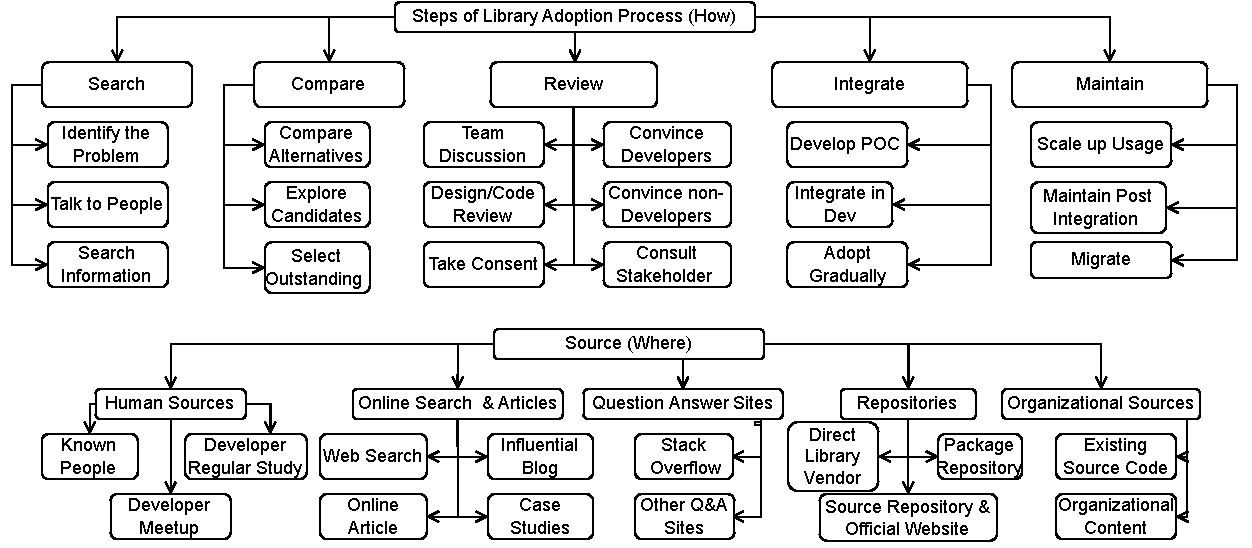
\includegraphics[scale=0.85]{images/process.pdf}
    \caption{Concepts related with library adoption process and relevant information sources}
    \label{fig:process}
\end{figure*}
% Using open coding and constant comparison of \td{24} interviews, we discovered total 83 library adoption concepts. By conducting axial coding, we categorized these concepts into 19 categories under 4 major categories of adoption steps, surrounding conditions, library specific factors, and information sources. Figure \ref{fig:taxonomy} shows the hierarchy of all 83 library adoption concepts. Numbers shown beside the major categories in Figure \ref{fig:taxonomy} refer to the total number of concepts under that category (e.g., 18 concepts under 'steps' category).
\subsubsection{Steps of Library Adoption (18)}
A third-party library can be adopted in 5 major steps starting from search for library information, and followed by comparing available libraries, reviewing the libraries along with other teammates or teams, integrating the library into the application, and finally maintaining the library throughout the process of the host application where it was integrated. Developers would \qi{search it in the Google, it will actually suggest few of the blogs or Stack Overflow community}{P04}, then compare factors among multiple libraries: \qi{you go to Stack Overflow and you find some articles there that refers to some of the libraries. From there you go into those libraries spaces and GitHub and then you take a look at it.}{P15} The library selected after comparative analysis can be further reviewed during code review or design review in case of an important feature since \qi{using a third-party library in any project is a major decision and that decision has to be reviewed by at least one or two senior developer as well.}{P14} Depending on the company size and practices, developers may request approval from dedicated teams who review the security and license issues of third-party libraries: \qi{So we have the DevOps team... they have a way to cheque the security also any vulnerability issue altogether and also if we are actually using it in the proper license.}{P11} 

The integration of library can also be a gradual process, since developers \qi{do some proof of concept for some libraries. Then for the adoption phase we normally take it slowly, like for example, when we want to introduce Hikary CP instead of Tomcat, we have to apply this library to one or two services, then gradually move to the wide adoption of that library.}{P01} For some important features, developers will need to keep the libraries updated to the latest versions because \qi{there is no limit on improvement... You can opt in for new versions or you can ignore the new versions. Usually major versions might have something which can break your code. But you don't upgrade without any reason.}{P05}

\subsubsection{Source of Information about Libraries (14)} Developers need to collect information about libraries for making the evaluation for adoption. The categories of sources developers use are human sources, online search engines and articles, question-answer sites, repositories, and organizational internal sources. After understanding a problem statement that may require libraries, \qi{the very first step before going to searching is I'm reaching out to my colleagues.}{P11} Some studious developers might also disagree that \qi{the first thing is not opinion from other people, rather from developer's daily study. Developers always look for [learning] things, right?}{P01} When people don't get help from peers, \qi{then probably Google search is the first thing to do.}{P03} When online search do not provide enough idea about the libraries, developers would go to popular question-answer sites: \qi{Stack Overflow is a huge resource for seeing what different people recommend... and also seen a lot on things like Quora and Reddit where you say what's the best library for doing X and people will list out a couple of different options there.}{P07}

To explore open source libraries, developers \qi{go to GitHub to see the code base and how it is maintained, how frequent the commits are coming, how frequent the issues are coming, when the last issue has been resolved, how long the issues are resolved?}{P01} Developers would also consider visiting programming language specific package repositories as \qi{Google for JavaScript based libraries [npmjs.com].}{P04} In addition to external knowledge sources, some organizations can have \qi{internal GitHub. Then there are internal search engines, also there are some question answer like Stack Overflow... I think that is true for all these big corporations.}{P02}

\subsection{Factors and Conditions influencing Process (RQ2)}
\begin{figure*}
    \centering
    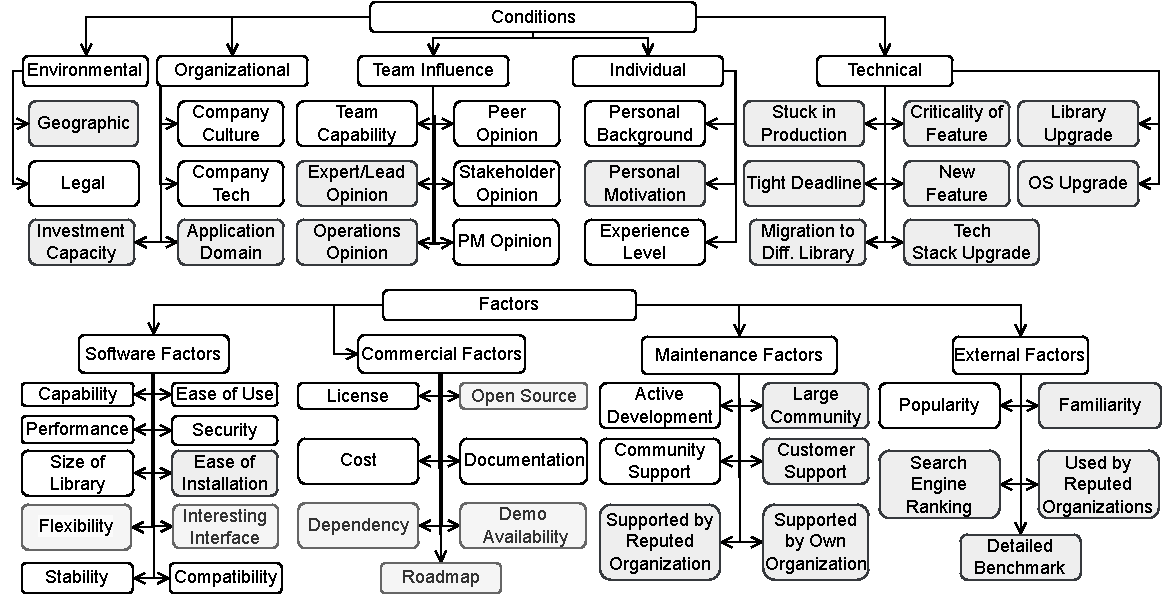
\includegraphics[scale=0.85]{images/conditions.pdf}
    \caption{Concepts related with factors and conditions influencing library adoption process}
    \label{fig:conditions}
\end{figure*}
Internal, external conditions and library specific factors impact the adoption process.

\subsubsection{Conditions of Library Adoption (23)}
Library adoption process can be influenced by environmental, organizational, team specific, individual, and technical scenario specific conditions and opinions. This conditions determine which factors or steps developers will consider. For example, developers will seriously consider compliance issues when there are strict regulatory requirements: \qi{in Germany you have to report a security breach in your company... you have to pay 2 percent of the revenue if a security breach happens and your data gets leaked.}{P17} Organizations can also enforce policies for library selection: \qi{the companies that are in the industry for long time, they almost always have this kind of guideline, training and tools that gets involved whenever you are choosing third-party libraries.}{P03}

Developers are often influenced by the opinions of fellow developers or technical experts since \qi{selection of library is always a team decision in a democratic way}{P10}. Sometimes, tech leaders will also consider the strength and conditions of their team: \qi{I went for Vue because most of the developers in my company were mostly back-end developers and I found Vue is very back-end developer friendly.}{P04} Individual developer's personal motivation can encourage them to choose reusable libraries more than their peers: \qi{The excitement of trying some new library was also fairly motivating to keep my skills up to date whereas a lot of people would just write their own solutions.}{P06} Project deadlines can also play important role how developers will choose a library: \qi{For example, if you gave me this [JSON parsing] problem and you said I need a prototype in a month, I would choose Gson. If you said latency and memory is important to me, I'll choose Jackson.}{P13} Moreover, \qi{if the feature is too business critical, then it goes through even rigorous decision making process than the other where, for example, you are just trying to choose a library to show an image and crop it. So that is not so business critical.}{P15}

\subsubsection{Factors of Library Selection Criteria (28)}
Developers evaluate third-party libraries on four major criteria which are software factors, commercial factors, maintenance factors, and external factors related to the specific library. Among the technical software application concerns, the first thing developer could is whether the library \qi{is meeting the requirements or not.}{P04} Moreover, \qi{developer usage is a very important important criteria}{P01} and developers might prefer libraries which are easy to install, easy to use with interesting interfaces. Developers would also consider performance, compatibility, and security aspects: \qi{we have to understand how much memory it is gonna use,... how much time it takes to execute? or how much CPU is gonna use? Is this library compatible with the development environment? how is the thread safety within the library?}{P15}

After the technical aspects of libraries, \qi{the next criteria is whether there is free or open source mostly}{P05} which are related with the commercial supply chain specific concerns that can also include documentation, demonstration, and roadmap of the libraries. Besides the technical and commercial factors, developers look for libraries developed by active contributors, backed by reputed organizations or large community since: \qi{no software or platform is bug free... if someone raises a bug, there has to be someone in the library side who needs to take care it and then needs to push the fix.}{P04} We also observed a common library selection criteria is popularity which varies from library to library: \qi{We cannot compare sixty million with one thousand downloads. So this library [with high download count] is obviously a choice.}{P04} Another such external criteria is developer's familiarity with a specific library since \qi{oftentimes what happens is that the decision or the choice gets influenced by individual’s bias or familiarity or previous experience with one particular product or service}{P08} 


\subsection{The Guiding Principles (RQ3)}
\label{sec:gp}

All concepts of library adoption process described in section \ref{sec:taxonomy} have complex interaction with the six guiding principles (GP). On the basis of internal and external conditions, certain advantages and disadvantages of libraries become eminent to developers and they follow guiding principles accordingly. The guiding principles then influence the selection criteria, process, and information sources: \qi{It's not that always you have to choose a library or framework which is technically the best. Rather capabilities of the library and the organization, the domain, the people, the timing, everything influences that decision.}{P01} 

During the theoretical integration of our study, the six guiding principles emerged from the benefits and baggage of libraries - why developers want to use a library and why they still remain cautious to use a library.

\begin{tcolorbox}[flushleft upper,boxrule=1pt,arc=0pt,left=0pt,right=0pt,top=0pt,bottom=0pt,colback=white,after=\ignorespacesafterend\par\noindent]
\textbf{Benefits of Libraries:} Few guiding principles are mostly motivated by the benefits libraries have to offer such as delivering faster and reusing a robust component for improved application quality.
\end{tcolorbox}

Figure \ref{fig:gp} provides exemplary interactions of each guiding principle with the adoption process concepts. For example, developers in a startup culture pressed by faster delivery would be happy to rip the benefit of using any existing third-party library to meet the deadline and may decide to follow the principle of 'Just Do It' and eventually find libraries which are easy to use, easy to install, popular in community, and familiar to them, and they would collect such information mostly from peer developers without going through much exploration. In the following subsections, we describe such interaction with each of the guiding principles.

\subsubsection{Just Do It} 
The most prominent benefit developers get out of third-party libraries is \qi{[the library] makes our \textbf{life simpler}. The application development definitely gets \textbf{faster} by using that.}{P15}. \qw{C}{Company culture}, organization's \qw{C}{investment capacity}, developer's \qw{C}{personal background} and \qw{C}{experience level}, and even \qw{C}{deadline of feature} can encourage developers to follow this guiding principle: \qi{For startups, a lot of it [priority] is just speed to market and how much resources is gonna eat up using any specific library.}{P07}

By following this guiding principle, developers would tend to rely on \qw{S}{known people} to collect information faster and gather recommendations: \qi{if you ask a friend, they can easily show you the shortcuts, right? You don't need to scroll for hours through the Stack Overflow to find the best solution.}{P11}

Developers may prefer libraries which are \qw{F}{easy to use} and \qw{F}{easy to install} to \qi{just import it and use the functions}{P11}. Developer may not be much concerned about long-term maintenance factors such as the \qw{F}{active development}, \qw{F}{community support}, \qw{F}{stability} issues of the library: \qi{It was going to solve a particular promotion or something, and it was going to be retired. So usually the long term maintainability was not a factor.}{P06}

\subsubsection{Reuse Robust Components} 
Third-party libraries are reusable components that significantly reduce \qi{boiler plate code}{P19} in software applications. \qw{C}{Experienced developers} \qi{don't reinvent the wheel. I want to use as much as already developed, tested and robust software into my solution... the main thing is that reusability and having stability in the application inherently out-of-the-box \textbf{by using a stable, robust library}}{P22} \qw{C}{Company culture} or large organizations can promote library usage: \qi{So [this large corporation] as a whole is actually built on the open source libraries that are suitable for our use cases. But that actually has been one of our primary focus as well. If you find a library, use it; only build if you can't find anything.}{P13} In certain \qw{C}{technology} stack, developers \qi{actually use third-party libraries all the time and it's a necessity when you're developing a mobile application. It's almost always a necessity to use third-party libraries.}{P14} 

When developers follow guiding principle of reusing robust components, they thoroughly check any option to reuse a library during \qw{P}{code/design review}: \qi{as a code reviewer or design reviewer, I try to pay attention to \textbf{don't repeat yourself principle that you don't want to write something that's already in a library.}}{P13} Also they would check \qw{S}{internal sources} for existing usage of a library: \qi{when you work on project or the product you usually work on existing code base, so I think the first thing to try out is to just stick to the existing [library]}{P02}

With this principle, developers in long term or complex products prefer to choose \qw{F}{stable} which are \qw{F}{actively maintained} for a long period and supported by with \qw{F}{large community}: \qi{with a project like ours [C++ code application developed over 27 years], the main time we adopt a library is when it is an implementation of a tech spec. OpenSSL, there's a tech spec for SSL. Here's a whole library that has been carefully implemented against the spec.}{P18}

\subsubsection{Improve Application Structure}
Improvement of application structure is a constant effort of software design architects. Veteran designers like P22 would take the opportunity to improve the architecture \qi{the moment you have to bring something in because there are new requirements is the time to assess how you've structured your application and does it still serve you and your customers or the business requirements you have. So that's the opportunity to look at the structural aspect of the application and make sure you do want to avoid changing it or maybe it's the time to change it.}{P22} Since libraries provide more flexibility that larger frameworks, developers would often prefer libraries in \qw{C}{technical scenarios} of large scale applications where the application has its own structure: \qi{just go with the smaller libraries that solve a very particular problem so that we have full control. But if we integrate with the framework then we always need to solve with that framework because we cannot go outside of that framework until we completely remove that framework}{P9}. 

While inspired by the principle of architectural improvement and consistency, architects would adopt third-party libraries when absolute necessary for specification driven most \qw{F}{popular} libraries. The project P18 worked was such an example where they had less than 20 libraries in a two million line source code. Even when they \qw{P}{integrate} libraries, they would wrap it under their own structure: \qi{We will create just a thin wrapper, that ends up looking like the rest of our platform. The simple source file [wrapper API] is protecting the two million lines of code from the idiosyncrasies of this one particular library.}{P18} By keeping third-party libraries modular, architects ensure that their application does not have critical \qw{F}{dependency} on external library: \qi{we attempt to make it very pluggable, like modular. So if I need to remove my dependency on third-party library X and swap in a different one, my design of my software is clean enough that I can do that without like having to overhaul.}{P22}

\subsubsection{Empower the Team} Adopting third-party libraries also empowers the development teams. Open source libraries provide developers working experience with popular development components to acquire transferable knowledge whereas proprietary solutions developed internally can create bottlenecks: \qi{When you move to using something that's an open source third-party solution, it's well documented, suddenly an entire team of people can help address a problem and your speed to fixing something goes from multiple days or weeks to hours. And you empower the whole team rather than an [internal] specialist who can't go on vacation because if she does, sorry, you're waiting.}{P22}

\qw{C}{Company Culture} plays the biggest role in driving the principle of empowering the team. \qw{C}{Tech leads' opinion} will regularly be influenced by the \qw{C}{capability of the development team}. While choosing libraries, developers will also consider \qw{C}{peer opinions}: \qi{I'm not taking a decision for myself. Also there are seniors in every organization who are more experienced and they may have some opinions on it.}{P01} When guided by the empowerment principle, developers would often discuss with peers during the library \qw{P}{review} phase: \qi{Let's say, I proposed one library from my previous work. And then I have to explain it to the team members.}{P10} While organizations empower teams by letting them adopt third-party libraries, the adoption also improves developers' transferable skills. Developers would not only look for \qw{F}{ease of use} in the libraries, but also attempt adopting \qw{F}{popular} libraries in the community: \qi{So looking at community popularity helps because then you can it helps to hire people. It helps to retain people. They like to use technologies that are transferable.}{P19}

\begin{tcolorbox}[flushleft upper,boxrule=1pt,arc=0pt,left=0pt,right=0pt,top=0pt,bottom=0pt,colback=white,after=\ignorespacesafterend\par\noindent]
\textbf{Baggage of Libraries.} Third-party libraries come with certain security and legal risks and life long maintenance burden in complex long term products: \qi{there can be flaw within the library that could introduce security flaw and attacks to your system. It is always, always risky when you build a core component on top of a library and the library is not getting developed.}{P15}
\end{tcolorbox}


\subsubsection{Ensure Compliance \mybarsbwa{7}{2}{2}{2}}
Besides privacy and security vulnerabilities, open source libraries can also come with legal risks, if developers are not careful about permissive (such as MIT, BSD) and restrictive licenses (such as GPL) \cite{website:osi} and the appropriate license for their application: \qi{we had a very bad experience with this. With the legacy system, we were using so many different libraries and there is a licensing issue and we had to replace half of the library. Otherwise we had to pay lots of money. So that's why we are now very, very concerned about adding any external library, because if we don't comply with the license, it will be a legal problem.}{P09}

However, not all development teams equally consider the impact of compliance issues. \qw{C}{Legal environment} of the organization or their customers are primary driver for compliance principle: \qi{Since we work with people from Europe, UK, US and other area and they have a very strong data security policy, we have to be confident that they're secure well.}{P04} Few \qw{C}{application domains} such as health, finance, media are also more regulated and require organizational policies for ensuring compliance.

Under such regulatory compliance concerns, developers would prefer \qw{F}{open source}, \qw{F}{secure} and compliant libraries: \qi{So there are libraries who advertise that they are already GDPR \cite{website:gdpr} compliant or FedRAMP \cite{website:fedramp} compliant. So those kinds of libraries are always preferred over libraries that don't have a clear signal.}{P19} Driven by this principle, developers would consider widely trusted and \qw{F}{popular} libraries so that any vulnerability information can be instantly available in global news and \qw{S}{online articles} during \qw{P}{post integration maintenance}: \qi{Because the open source libraries get far more scrutiny, they tend to get better maintenance, they get pounded on. You hear about the security vulnerabilities and you can respond to them... We're looking for a library that has been used for five years, ten years, and that's in open source, broad acceptance and excellent track record and continuing maintenance. OpenSSL is a perfect example of that.}{P18} To protect themselves from legal and \qw{F}{license} concerns, \qi{the big companies almost always have tools and processes that the engineers must follow when they are trying to integrate one library.}{P03}

%\begin{enumerate}[wide, labelwidth=!, labelindent=0pt]
\subsubsection{Maintain Continuous Stability}
Other than compliance issues, the biggest risk of using a third-party library occurs \qi{if the contributors are gone in those third-party libraries repositories, suddenly the whole production application is broken}{P10}. Developers will also need engage resources to upgrade libraries without breaking there existing application: \qi{when we integrated the updated version our whole interface broke. And we had to change a lot of code, all the interceptors, interfaces, everything... This maintenance is quite hard. It's actually a full time work to always keep updated, to always stay updated.}{P14}

Maintenance and upgradation of third-party libraries can be sometimes enforced by \qw{C}{company culture} in matured organization: \qi{So there is internal processes that look for freshness. And they will notify you when you're getting outdated. Every library has designated set of owners. So it's the owner's job to make sure that they comply with the update requirements.}{P19} Certain \qw{C}{application domains} such as mobile applications are more susceptible to library upgradation because of yearly change of operating systems: \qi{In Android, it's a little bit less problematic because Google provides backwards compatibility for a lot longer... It's just the difference between how Apple does it, where in the second year they may mark the application just obsolete.}{P20}

To protect themselves from abandonment and stability risks, developers would look for libraries where \qw{F}{large community} and contributors are involved. To \qw{P}{search information} about \qw{F}{active development}, they would check \qw{S}{source repositories}: \qi{we have to check that whether this library maintenance are active or not. We can determine that by checking their GitHub repository when was the last push was given?}{P04} Developers would also prefer libraries \qw{F}{supported by reputed organizations} because \qi{they have less chances to disappear. For example, the libraries backed by Google or by Facebook, we can hope that they will not easily disappear.}{P14} Finally, developers will be continuously engaged to check if any new version needs to be upgraded or not: \qi{using old libraries is going to be a really big issue. So in my works, of course, I try to update it as soon as I can to make it compatible with new systems.}{P23}

\textbf{Summary Impact of Guiding Principles.} As we have described the interaction of guiding principles with library adoption process concepts, we also mapped each concept with the relevant guiding principle. Figure \ref{fig:Concept-Principle-Heatmap} shows a summary of impacts by the principles on the concept categories. For example, GP1: Just Do It principle has interaction with highest 46 total concepts whereas it influences (either positively or negatively) 6 review actions (e.g., under Just Do It, developers may not perform thorough code/redesign review, or take expert consent) and 6 software factors. Though GP4: Empower the Team has lowest total impact on 13 concepts, it has most impact again on the review process and team influence.

Finally, it must be noted that the conditions do not come in isolation, and guiding principles also do not activate exclusively. Rather in practical scenarios, developers are always facing multiple, even conflicting situations, and balancing among guiding principles to make their final decisions.

%Experienced developers would be willing to use a proven library by following guiding principle 'Reuse Robust Component' and find libraries with better stability, higher performance, and thoroughly compare candidate libraries, and also collect library related information from source code repositories and trusted blogs.
\begin{figure}
    \centering
    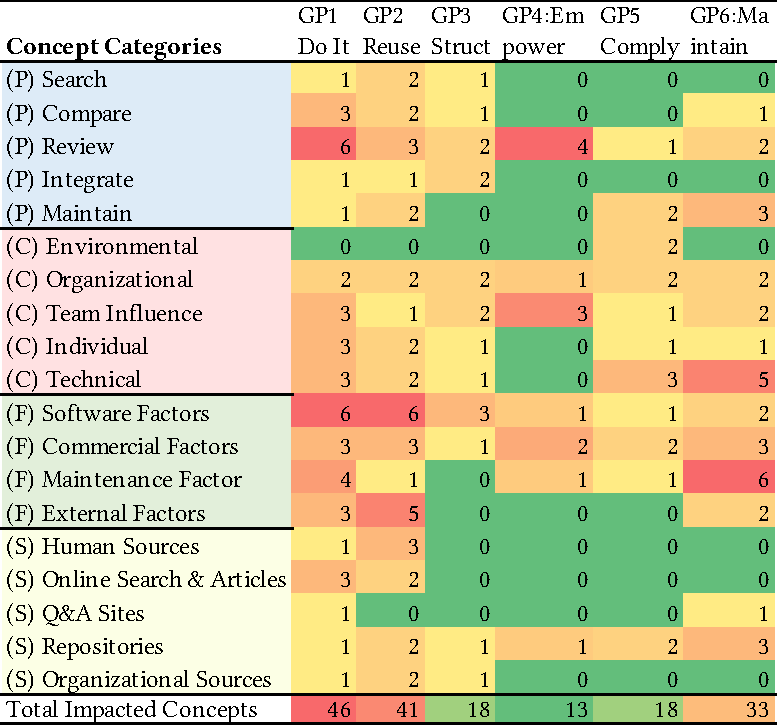
\includegraphics[scale=0.7]{images/Concept-Principle-Heatmap.pdf}
    \caption{Heatmap based on the number of concepts impacted by each guiding principle (GP1 to GP13). For example, 2 concepts from Individual category is impacted by GP1-Just Do It. The more red means more concepts under that category is impacted by the corresponding GP. (C), (F), (P), (S) denotes tertiary concept categories Conditions, Factors, Steps, and Sources respectively.}
    \label{fig:Concept-Principle-Heatmap}
\end{figure}

%Numbers aligned with the text:  \circled{C} \circled{F} \circled{P} \circled{S} end.


